\subsection{Graph coloring}

The four color theorem was initially formulated from a problem in coloring world maps. A map consists of regions that can border other regions on a flat surface. When we talk about a \textit{coloring} of a map, we mean a way to color its regions such that any two neighbors are colored differently.

The actual shape of the regions in our map is not of importance here. The key information that is needed from a map, is the connectivity between regions. Such information can be represented in a \textit{graph} where vertices (circles) correspond to regions. An edge between two vertices then indicates that the two corresponding regions are neighbors.

\begin{figure}[!h]
    \centering
    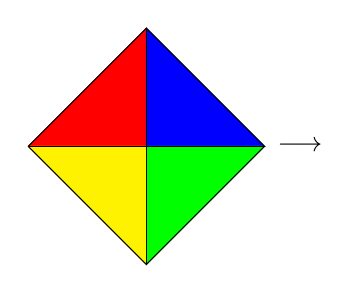
\begin{tikzpicture}[scale=1.5]
        \coordinate (v1) at (-1, 0);
        \coordinate (v2) at (0, 1);
        \coordinate (v3) at (1, 0);
        \coordinate (v4) at (0, -1);
        \coordinate (c) at (0, 0);

        \draw [fill, red] (v1) -- (v2) -- (c) -- (v1);
        \draw [fill, blue] (v2) -- (v3) -- (c) -- (v2);
        \draw [fill, green] (v3) -- (v4) -- (c) -- (v3);
        \draw [fill, yellow] (v4) -- (v1) -- (c) -- (v4);
        \draw (v1) -- (v2) -- (v3) -- (v4) -- (v1);
        \draw (c) -- (v1);
        \draw (c) -- (v2);
        \draw (c) -- (v3);
        \draw (c) -- (v4);
        \node at (1.3, 0) { $\longrightarrow$ };
    \end{tikzpicture} 
    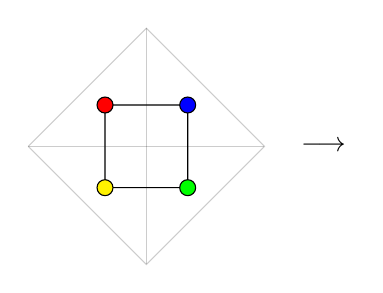
\begin{tikzpicture}[scale=1.5]
        \coordinate (v1) at (-1, 0);
        \coordinate (v2) at (0, 1);
        \coordinate (v3) at (1, 0);
        \coordinate (v4) at (0, -1);
        \coordinate (c) at (0, 0);

        \node[circle, fill, scale=0.01cm, red, draw=black] (m1) at (-0.35, 0.35) { $v_1$ };
        \node[circle, fill, scale=0.01cm, blue, draw=black] (m2) at (0.35, 0.35) { $v_2$ };
        \node[circle, fill, scale=0.01cm, green, draw=black] (m3) at (0.35, -0.35) { $v_3$ };
        \node[circle, fill, scale=0.01cm, yellow, draw=black] (m4) at (-0.35, -0.35) { $v_4$ };

        \draw (m1) -- (m2) -- (m3) -- (m4) -- (m1);
        \draw[opacity=0.2] (v1) -- (v2) -- (v3) -- (v4) -- (v1);
        \draw[opacity=0.2] (c) -- (v1);
        \draw[opacity=0.2] (c) -- (v2);
        \draw[opacity=0.2] (c) -- (v3);
        \draw[opacity=0.2] (c) -- (v4);
        \node at (1.5, 0) { $\longrightarrow$ };
    \end{tikzpicture}  
    \begin{tikzpicture}[scale=1.5, mid arrow/.style={
        postaction={ decorate, decoration={ markings, mark=at position 0.6 with { \arrow[black]{>>} } } } }]
        \coordinate (v1) at (-1, 0);
        \coordinate (v2) at (0, 1);
        \coordinate (v3) at (1, 0);
        \coordinate (v4) at (0, -1);
        \coordinate (c) at (0, 0);

        \node[circle, fill, scale=0.015cm, label=above left:$a$] (m1) at (-0.35, 0.35) { };
        \node[circle, fill, scale=0.015cm, label=above right:$b$] (m2) at (0.35, 0.35) { };
        \node[circle, fill, scale=0.015cm, label=below right:$c$] (m3) at (0.35, -0.35) { };
        \node[circle, fill, scale=0.015cm, label=below left:$d$] (m4) at (-0.35, -0.35) { };

        \draw[mid arrow] (m1) -- (m2);
        \draw (m2) -- (m3) -- (m4) -- (m1);
        \draw[opacity=0.0] (v1) -- (v2) -- (v3) -- (v4) -- (v1);
    \end{tikzpicture}      
    \caption{The translation of a map coloring to a graph coloring. In the last step we replace colors by the letters $a$,$b$,$c$ and $d$ for convenience. We obtain the coloring called $abcd$. The edge $\gg$ indicates the order of the coloring in case of ring-shaped graphs. }
    \label{fig:colortut}
\end{figure}

From now on, we will leave the notion of maps and regions behind us and work solely with graphs. The four color theorem can then be formulated as follows.

\begin{theorem}
    Every planar graph can be colored in at most four colors.
\end{theorem}

With \textit{planar graph} we mean a drawing of a graph as in the left-most graph of Figure \ref{fig:colortut}. Edges are not allowed to cross each other. The proof of this theorem required over a 100 years to complete, despite its simple statement. What would you do to prove such a statement? You would first try very hard for one day. After that, you move on to a weaker variant of the statement. This brings us to the five color theorem.